%! Author = avime
%! Date = 4/18/2020

\documentclass[12pt,paper=letter]{scrartcl}

\usepackage[page,center,titling,header,footer,links]{worksheet}

\addtolength{\jot}{1em}

\begin{document}

    \title{Electrostatics}
    \author{Avi Mehra}
    \date{4/18/2020}
    \maketitle


    \section{What is electrostatics?}\label{sec:what-is-electrostatics?}
    \bluebf{Electrostatics is the study of non-moving electricity.}
    \pnp
    Our lives depend on electricity, or the property of being electrically charged.
    \pnp
    Especially if you did the Electric House project in Physics, you probably believe that electricity is the motion of electrons through a conductive material.
    This is true, but electricity is more than just moving electrons.
    \pnp
    You might have heard the term \emph{static electricity} to describe what happens when electrically charged objects cause forces without moving.
    This \emph{static electricity} is what we will be studying in Electrostatics.
    We will focus on the following topics:

    \begin{itemize}[topsep=2pt,itemsep=-0.7ex,partopsep=1ex,parsep=1ex]
        \item Electric charge
        \item Electric potential
        \item Potential difference (voltage)
        \item Electric fields
        \item Electric force (Coulomb's Law)
        \item Potential energy
    \end{itemize}

    \subsubsection{About this worksheet}
    Some of the practice problems and exercises will have hints like the one at the end of this paragraph.
    You can view the hints at the end of this worksheet (Section~\ref{sec:hints}), or by clicking the number in the hint. \hint{\ref{hint:ex}}

    \pnp

    If you still need help after the hints,
    you can contact us through email, class/office hours, or the tutor request form on the \href{https://tiny.cc/shieh/grades}{Grades page} of the \href{https://tiny.cc/shieh}{class website}.
    \pnp
    In this worksheet, we will ignore significant figures and use either 0 or 1 digit after the decimal point.
    Electric potential and potential energy are treated as relative to a point at infinity.
    If you don't know what these mean, don't worry.
    %\subsection{Terminology}
    %\bluebf{Magnitude:} this is the numeric value of


    \section{Electric Charge}\label{sec:electric-charge}
    Think of some object, for example your phone or a desk.
    This object has properties like color, volume, mass, and density.
    \pnp
    Electric charge is similar to mass;
    it's the amount of ``substance" that an object has.
    Mass is the amount of matter in an object;
    electric charge is the amount of ``electricity" that an object has.
    \pnp
    Later we will learn that, because of this fact, gravity and electricity are very similar.

    \begin{exboxed}[Mass]
        My phone has a mass of $184\text{ g}=0.184\text{ kg}$.
        As long as I don't break off a piece of the phone, its mass will stay the same.
    \end{exboxed}


    \begin{exboxed}[Electric charge]
        A proton has a charge of $1.6021766208 \times 10^{-19}$ Coulombs.
        The proton will always have the same charge.
    \end{exboxed}


    \section{Electrostatic (Electric) Potential}\label{sec:electrostaticpotential}

    \subsection{Analogy\textemdash Gravitational Potential}\label{subsec:gravitational-potential}

    Think about a ball being dropped from a tower (Figure~\ref{fig:ball_tower}).
    When the ball is high, gravity can push it down.
    Once the ball is on the ground, gravity can't force it down anymore.
    When the object is high up, it is in high potential, and when it is on the ground, it is in a state of 0 potential.
    In Figure~\ref{fig:tower}, you can see that gravitational potential increases with height.
    For gravity, potential is a constant multiple of height:
    \[\text{Potential}=g\cdot h.\]

    \begin{figure}
    \centering
    
\includegraphics[width=.5\textwidth]{ball_tower.jpg}
    \caption{A children's toy with balls at different heights.
    The potential is highest at Level 1 and keeps decreasing until it is zero at Level 5.
    Image from Bobykids Store on AliExpress.
        \cite{aliexpress}}
    \label{fig:ball_tower}
\end{figure}

    \begin{figure}
    \centering

    % Gradient Info

\tikzset {_cb29xqt9q/.code = {\pgfsetadditionalshadetransform{ \pgftransformshift{\pgfpoint{0 bp } { 0 bp }  }  \pgftransformrotate{-90 }  \pgftransformscale{2 }  }}}
\pgfdeclarehorizontalshading{_xqd1d5nx2}{150bp}{rgb(0bp)=(0.49,0.83,0.13);
rgb(37.5bp)=(0.49,0.83,0.13);
rgb(62.5bp)=(1,1,1);
rgb(100bp)=(1,1,1)}
\tikzset{every picture/.style={line width=0.75pt}} %set default line width to 0.75pt

\begin{tikzpicture}[x=0.75pt,y=0.75pt,yscale=-1,xscale=1]
%uncomment if require: \path (0,300); %set diagram left start at 0, and has height of 300

%Shape: Can [id:dp4097434097565138]
    \path  [shading=_xqd1d5nx2,_cb29xqt9q] (497,47.6) -- (497,249.6) .. controls (497,254.57) and (483.57,258.6) .. (467,258.6) .. controls (450.43,258.6) and (437,254.57) .. (437,249.6) -- (437,47.6) .. controls (437,42.63) and (450.43,38.6) .. (467,38.6) .. controls (483.57,38.6) and (497,42.63) .. (497,47.6) .. controls (497,52.57) and (483.57,56.6) .. (467,56.6) .. controls (450.43,56.6) and (437,52.57) .. (437,47.6) ; % for fading
    \draw   (497,47.6) -- (497,249.6) .. controls (497,254.57) and (483.57,258.6) .. (467,258.6) .. controls (450.43,258.6) and (437,254.57) .. (437,249.6) -- (437,47.6) .. controls (437,42.63) and (450.43,38.6) .. (467,38.6) .. controls (483.57,38.6) and (497,42.63) .. (497,47.6) .. controls (497,52.57) and (483.57,56.6) .. (467,56.6) .. controls (450.43,56.6) and (437,52.57) .. (437,47.6) ; % for border


% Text Node
    \draw (505,61) node [anchor=north west][inner sep=0.75pt]   [align=left] {High potential};
% Text Node
    \draw (505,184) node [anchor=north west][inner sep=0.75pt]   [align=left] {Low potential};
% Text Node
    \draw (505,233) node [anchor=north west][inner sep=0.75pt]   [align=left] {Zero potential};


\end{tikzpicture}

    \caption{A tower with multiple stories.
    Gravitational potential increases as you move upwards.
    The darker the color, the more potential at that height.}
    \label{fig:tower}
\end{figure}

    \subsection{Electric Potential}\label{subsec:electric-potential}
    In Subsection~\ref{subsec:gravitational-potential},
    we found out that gravitational potential is just a (scaled) measure of height, or how much gravity can make an object move.
    Electric potential is very similar; \bluebf{it is a measure of how much the electric force can make an object move}.
    \pnp
    Electric potential is caused by electrically charged objects,
    just like gravitational potential is caused by gravitationally charged objects (the Earth).

    \begin{figure}
    \centering

    \tikzset {_efbsk5dva/.code = {\pgfsetadditionalshadetransform{ \pgftransformshift{\pgfpoint{89.1 bp } { -128.7 bp }  }  \pgftransformscale{1.32 }  }}}
    \pgfdeclareradialshading{_ah1a1en88}{\pgfpoint{-72bp}{104bp}}{rgb(0bp)=(1,1,1);
    rgb(0bp)=(1,1,1);
    rgb(25bp)=(0.48,0.15,0.15);
    rgb(400bp)=(0.48,0.15,0.15)}
    \tikzset{every picture/.style={line width=0.75pt}} %set default line width to 0.75pt

    \begin{tikzpicture}[x=0.75pt,y=0.75pt,yscale=-1,xscale=1]
%uncomment if require: \path (0,300); %set diagram left start at 0, and has height of 300

%Shape: Circle [id:dp9020583883547655]
        \path  [shading=_ah1a1en88,_efbsk5dva] (93,220) .. controls (93,206.19) and (104.19,195) .. (118,195) .. controls (131.81,195) and (143,206.19) .. (143,220) .. controls (143,233.81) and (131.81,245) .. (118,245) .. controls (104.19,245) and (93,233.81) .. (93,220) -- cycle ; % for fading
        \draw   (93,220) .. controls (93,206.19) and (104.19,195) .. (118,195) .. controls (131.81,195) and (143,206.19) .. (143,220) .. controls (143,233.81) and (131.81,245) .. (118,245) .. controls (104.19,245) and (93,233.81) .. (93,220) -- cycle ; % for border

%Straight Lines [id:da31486330865489753]
        \draw    (141.3,206) -- (263.56,135.99) ;
        \draw [shift={(265.3,135)}, rotate = 510.21] [color={rgb, 255:red, 0; green, 0; blue, 0 }  ][line width=0.75]    (10.93,-3.29) .. controls (6.95,-1.4) and (3.31,-0.3) .. (0,0) .. controls (3.31,0.3) and (6.95,1.4) .. (10.93,3.29)   ;
%Shape: Circle [id:dp26251024335558126]
        \draw  [fill={rgb, 255:red, 0; green, 0; blue, 0 }  ,fill opacity=1 ] (274.24,128.58) .. controls (274.11,126.22) and (275.92,124.22) .. (278.28,124.11) .. controls (280.64,124.01) and (282.67,125.84) .. (282.8,128.2) .. controls (282.93,130.56) and (281.13,132.56) .. (278.76,132.67) .. controls (276.4,132.77) and (274.38,130.94) .. (274.24,128.58) -- cycle ;

% Text Node
        \draw (107,210) node [anchor=north west][inner sep=0.75pt]  [font=\Large] [align=left] {$\displaystyle Q$};
% Text Node
        \draw (284.8,131.2) node [anchor=north west][inner sep=0.75pt]   [align=left] {Point $P$};
% Text Node
        \draw (180,154) node [anchor=north west][inner sep=0.75pt]  [font=\LARGE,rotate=-330.07] [align=left] {$\displaystyle r$};


    \end{tikzpicture}
    \caption{A point $P$ at a distance $r$ from a charge $Q$.}
    \label{fig:potential}
\end{figure}

    % Law, definition, formula
    \begin{thmboxed}
        \label{thm:potential}
        The electric potential $V$ caused by a charge of $Q$ at a distance of $r$ away
        (the potential at Point $P$ in Figure~\ref{fig:potential}) is given by
        \begin{equation}
            V=\frac{kQ}{r},
            \label{eq:potential}
        \end{equation}
        where $k$ is a constant $\approx\kconst$.
    \end{thmboxed}

    It is important to note that both gravitational and electric potential are properties of space (related to position),
    not of any object sitting within space.

    %   \begin{exboxed}
    %      What is the electric potential ten meters ($10 \meters$) from a positive charge of twenty Coulombs ($+20\coulombs$)?
    % \end{exboxed}

    \begin{exboxed}
        \label{ex:potential_1}
        What is the electric potential $10 \meters$ from a charge of $+20\coulombs$?
    \end{exboxed}

    To solve this problem we can just use the formula from Theorem~\ref{thm:potential}:
    \begin{align*}
        V&=\frac{kQ}{r}\\
        &=\frac{\del{\kconst}\del{20 \coulombs}}{10 \meters}\\
        &=\boxed{1.8\times 10^{10}\volts}.
    \end{align*}

    \begin{exboxed}
        The electric potential at a point three meters ($3\meters$) from a charge is -1 Volt ($-1\volts$).
        What is the value of the charge?
    \end{exboxed}

    We begin as before, first plugging in the values that we know into Equation~\ref{eq:potential}:
    \begin{align*}
        V&=\frac{kQ}{r}\\
        -1\volts&=\frac{\del{\kconst}\del{Q}}{3 \meters},
    \end{align*}
    but now we have to make some manipulations.
    First, we multiply both sides of the equation by $3\meters$ to remove it from the denominator (the bottom):
    \begin{align*}
        -1\volts\cdot 3\meters&=\frac{\del{\kconst}\del{Q}}{3 \meters}\cdot 3 \meters\\
        -3 \volts\cdot\meter&=\del{\kconst}\del{Q}.
    \end{align*}
    We now divide by $k=\kconst$ so that we are left with $Q$,
    the charge that we want to find.
    \begin{align*}
        \frac{-3 \volts\cdot\meter}{\del{\kconst}}&=\frac{\del{\kconst}\del{Q}}{\del{\kconst}}\\
        -3.3\times 10^{-10} \coulombs &= Q\\
        Q &= \boxed{-3.3\times 10^{-10} \coulombs}.
    \end{align*}
    \begin{mdframed}[style=exmdbox]
        \begin{problem}
            What is the voltage at a point $7\meters$ from a $-2.2\coulombs$ charge?
        \end{problem}
        \begin{problem}
            What is the voltage $2\millimeters$ from a charge of $6.4\nanocoulombs$? \hint{\ref{hint:table_of_conversions}}
        \end{problem}

        \begin{problem}
            What happens to electric potential as the distance to the charge increases? \hint{\ref{hint:approximate_limit}}
        \end{problem}

        \begin{problem}[Shieh]
            The electric potential at a point $5\meters$ from a charge $Q$ is $1.48\times10^{11} \volts$.
            What is the charge $Q$?
        \end{problem}

        \begin{problem}[Challenge]
            An unknown charge is some unknown distance away from Point $P$.
            The electric potential at Point $P$ is $5 \volts\meter$ (Volt-meters) divided by the distance to the charge.
            What is the value of the charge? \hint{\ref{hint:voltage_challenge_1}}
        \end{problem}

    \end{mdframed}

    \subsubsection{Superposition}

    So far, we have looked at electric potential caused by one charged object.
    What happens when you add more?

    \pnp

    Electric potential obeys the \emph{Principle of Superposition},
    which means that you can add them together.
    An example will make this more clear.

    \begin{figure}[!ht]
    \centering

    \tikzset {_todkg7j90/.code = {\pgfsetadditionalshadetransform{ \pgftransformshift{\pgfpoint{89.1 bp } { -128.7 bp }  }  \pgftransformscale{1.32 }  }}}
\pgfdeclareradialshading{_brpskaxpq}{\pgfpoint{-72bp}{104bp}}{rgb(0bp)=(1,1,1);
rgb(0bp)=(1,1,1);
rgb(25bp)=(0.49,0.83,0.13);
rgb(400bp)=(0.49,0.83,0.13)}

% Gradient Info

\tikzset {_8vthb5elb/.code = {\pgfsetadditionalshadetransform{ \pgftransformshift{\pgfpoint{89.1 bp } { -128.7 bp }  }  \pgftransformscale{1.32 }  }}}
\pgfdeclareradialshading{_q7iq398zh}{\pgfpoint{-72bp}{104bp}}{rgb(0bp)=(1,1,1);
rgb(0bp)=(1,1,1);
rgb(25bp)=(0.96,0.65,0.14);
rgb(400bp)=(0.96,0.65,0.14)}

% Gradient Info

\tikzset {_5q0b6tgh9/.code = {\pgfsetadditionalshadetransform{ \pgftransformshift{\pgfpoint{89.1 bp } { -128.7 bp }  }  \pgftransformscale{1.32 }  }}}
\pgfdeclareradialshading{_f2f473rbw}{\pgfpoint{-72bp}{104bp}}{rgb(0bp)=(1,1,1);
rgb(0bp)=(1,1,1);
rgb(25bp)=(0.74,0.06,0.88);
rgb(400bp)=(0.74,0.06,0.88)}
\tikzset{every picture/.style={line width=0.75pt}} %set default line width to 0.75pt

\begin{tikzpicture}[x=0.75pt,y=0.75pt,yscale=-1,xscale=1]
%uncomment if require: \path (0,300); %set diagram left start at 0, and has height of 300

%Shape: Circle [id:dp16269792186593102]
    \path  [shading=_brpskaxpq,_todkg7j90] (113,133) .. controls (113,119.19) and (124.19,108) .. (138,108) .. controls (151.81,108) and (163,119.19) .. (163,133) .. controls (163,146.81) and (151.81,158) .. (138,158) .. controls (124.19,158) and (113,146.81) .. (113,133) -- cycle ; % for fading
    \draw   (113,133) .. controls (113,119.19) and (124.19,108) .. (138,108) .. controls (151.81,108) and (163,119.19) .. (163,133) .. controls (163,146.81) and (151.81,158) .. (138,158) .. controls (124.19,158) and (113,146.81) .. (113,133) -- cycle ; % for border

%Straight Lines [id:da7734881847924964]
    \draw [color={rgb, 255:red, 106; green, 187; blue, 17 }  ,draw opacity=1 ]   (161.3,119) -- (283.56,48.99) ;
    \draw [shift={(285.3,48)}, rotate = 510.21] [color={rgb, 255:red, 106; green, 187; blue, 17 }  ,draw opacity=1 ][line width=0.75]    (10.93,-3.29) .. controls (6.95,-1.4) and (3.31,-0.3) .. (0,0) .. controls (3.31,0.3) and (6.95,1.4) .. (10.93,3.29)   ;
%Shape: Circle [id:dp3011729282954776]
    \draw  [fill={rgb, 255:red, 0; green, 0; blue, 0 }  ,fill opacity=1 ] (294.24,41.58) .. controls (294.11,39.22) and (295.92,37.22) .. (298.28,37.11) .. controls (300.64,37.01) and (302.67,38.84) .. (302.8,41.2) .. controls (302.93,43.56) and (301.13,45.56) .. (298.76,45.67) .. controls (296.4,45.77) and (294.38,43.94) .. (294.24,41.58) -- cycle ;
%Shape: Circle [id:dp023330508474848743]
    \path  [shading=_q7iq398zh,_8vthb5elb] (413.61,154.56) .. controls (413.36,140.75) and (424.35,129.36) .. (438.16,129.11) .. controls (451.96,128.86) and (463.36,139.85) .. (463.61,153.65) .. controls (463.86,167.46) and (452.87,178.85) .. (439.06,179.1) .. controls (425.26,179.35) and (413.87,168.36) .. (413.61,154.56) -- cycle ; % for fading
    \draw   (413.61,154.56) .. controls (413.36,140.75) and (424.35,129.36) .. (438.16,129.11) .. controls (451.96,128.86) and (463.36,139.85) .. (463.61,153.65) .. controls (463.86,167.46) and (452.87,178.85) .. (439.06,179.1) .. controls (425.26,179.35) and (413.87,168.36) .. (413.61,154.56) -- cycle ; % for border

%Straight Lines [id:da14629502647663206]
    \draw [color={rgb, 255:red, 245; green, 156; blue, 35 }  ,draw opacity=1 ][fill={rgb, 255:red, 245; green, 166; blue, 35 }  ,fill opacity=1 ]   (417.3,131.2) -- (310.91,53.38) ;
    \draw [shift={(309.3,52.2)}, rotate = 396.18] [color={rgb, 255:red, 245; green, 156; blue, 35 }  ,draw opacity=1 ][line width=0.75]    (10.93,-3.29) .. controls (6.95,-1.4) and (3.31,-0.3) .. (0,0) .. controls (3.31,0.3) and (6.95,1.4) .. (10.93,3.29)   ;
%Shape: Circle [id:dp3372508230198279]
    \path  [shading=_f2f473rbw,_5q0b6tgh9] (147,269) .. controls (147,255.19) and (158.19,244) .. (172,244) .. controls (185.81,244) and (197,255.19) .. (197,269) .. controls (197,282.81) and (185.81,294) .. (172,294) .. controls (158.19,294) and (147,282.81) .. (147,269) -- cycle ; % for fading
    \draw   (147,269) .. controls (147,255.19) and (158.19,244) .. (172,244) .. controls (185.81,244) and (197,255.19) .. (197,269) .. controls (197,282.81) and (185.81,294) .. (172,294) .. controls (158.19,294) and (147,282.81) .. (147,269) -- cycle ; % for border

%Straight Lines [id:da030140594007627808]
    \draw [color={rgb, 255:red, 156; green, 16; blue, 224 }  ,draw opacity=1 ]   (186.3,244.2) -- (293.3,57.93) ;
    \draw [shift={(294.3,56.2)}, rotate = 479.88] [color={rgb, 255:red, 156; green, 16; blue, 224 }  ,draw opacity=1 ][line width=0.75]    (10.93,-3.29) .. controls (6.95,-1.4) and (3.31,-0.3) .. (0,0) .. controls (3.31,0.3) and (6.95,1.4) .. (10.93,3.29)   ;

% Text Node
    \draw (123,123) node [anchor=north west][inner sep=0.75pt]  [font=\Large] [align=left] {$\displaystyle Q_{1}$};
% Text Node
    \draw (304.8,18.2) node [anchor=north west][inner sep=0.75pt]   [align=left] {Point P};
% Text Node
    \draw (188.99,57.01) node [anchor=north west][inner sep=0.75pt]  [font=\LARGE,color={rgb, 255:red, 106; green, 187; blue, 17 }  ,opacity=1 ,rotate=-330.07] [align=left] {$\displaystyle r_{1}$};
% Text Node
    \draw (423.34,144.38) node [anchor=north west][inner sep=0.75pt]  [font=\Large,rotate=-358.96] [align=left] {$\displaystyle Q_{3}$};
% Text Node
    \draw (380.52,57.74) node [anchor=north west][inner sep=0.75pt]  [font=\LARGE,color={rgb, 255:red, 245; green, 156; blue, 35 }  ,opacity=1 ,rotate=-35.56] [align=left] {$\displaystyle r_{3}$};
% Text Node
    \draw (157,259) node [anchor=north west][inner sep=0.75pt]  [font=\Large] [align=left] {$\displaystyle Q_{2}$};
% Text Node
    \draw (190.12,157.06) node [anchor=north west][inner sep=0.75pt]  [font=\LARGE,color={rgb, 255:red, 167; green, 16; blue, 224 }  ,opacity=1 ,rotate=-300.83] [align=left] {$\displaystyle r_{2}$};


\end{tikzpicture}

    \caption{Three charges at different distances from a point $P$.}
    \label{fig:superposition}
\end{figure}


    \pnp

    In Figure~\ref{fig:superposition},
    we have three charges instead of one, and we want to calculate the potential at Point $P$.
    Now if we only had one charge, this would be easy;
    we could just use Equation~\ref{eq:potential} like we did in Example~\ref{ex:potential_1}.

    \begin{thmboxed}[Superposition]
        The electric potential caused by multiple charges is the sum of the electric fields caused by each charge.
        For example, with 3 charges as in Figure~\ref{fig:superposition},
        \begin{equation}
            V=V_1+V_2+V_3=\frac{kQ_1}{r_1}+\frac{kQ_2}{r_2}+\frac{kQ_3}{r_3}.
            \label{eq:superposition}
        \end{equation}
        More generally,
        \begin{equation}
            V = \sum_i V_i = \sum_i \frac{kQ_i}{r_i},
            \label{eq:advanced_superposition}
        \end{equation}
        but you won't need to know this for the assessment.
    \end{thmboxed}
    \begin{exrboxed}
        \label{exr:superposition}
        What is the potential at a point which is $1.3\centimeters$ from a $1\nanocoulombs$ charge, $2\centimeters$ from a $2.1 \nanocoulombs$ charge, and $9.1\millimeters$ from a $-10\nanocoulombs$ charge?
        \hint{\ref{hint:table_of_conversions}}
    \end{exrboxed}


    \section{Voltage and potential difference} \label{sec:voltage-and-potential-difference}
    Voltage is simply the difference, or change, of electric potential between two points in space.
    You might have heard voltage related to a battery;
    it is the difference in electric potential between the two ends of the battery.
    \pnp
    Voltage is represented as $\Delta V = V_b - V_a$ for the voltage between two points $a$ and $b$.
    You might also see this as $\Delta V_{ab}$ to make the direction of
    voltage more clear. \bluebf{Order matters.}

    \subsubsection{Particles moving in a potential difference}\label{subsec:potential-difference}
    \begin{figure}
    \centering

    \tikzset{every picture/.style={line width=0.75pt}} %set default line width to 0.75pt        

\begin{tikzpicture}[x=0.75pt,y=0.75pt,yscale=-1,xscale=1]
%uncomment if require: \path (0,300); %set diagram left start at 0, and has height of 300

%Rounded Rect [id:dp26809755411510916] 
    \draw  [fill={rgb, 255:red, 0; green, 0; blue, 0 }  ,fill opacity=1 ] (100,75.24) .. controls (100,74) and (101,73) .. (102.24,73) -- (359.06,73) .. controls (360.3,73) and (361.3,74) .. (361.3,75.24) -- (361.3,81.96) .. controls (361.3,83.2) and (360.3,84.2) .. (359.06,84.2) -- (102.24,84.2) .. controls (101,84.2) and (100,83.2) .. (100,81.96) -- cycle ;
%Rounded Rect [id:dp7927549373308511] 
    \draw  [fill={rgb, 255:red, 0; green, 0; blue, 0 }  ,fill opacity=1 ] (100,212.24) .. controls (100,211) and (101,210) .. (102.24,210) -- (359.06,210) .. controls (360.3,210) and (361.3,211) .. (361.3,212.24) -- (361.3,218.96) .. controls (361.3,220.2) and (360.3,221.2) .. (359.06,221.2) -- (102.24,221.2) .. controls (101,221.2) and (100,220.2) .. (100,218.96) -- cycle ;
%Straight Lines [id:da2975639375446937] 
    \draw [color={rgb, 255:red, 189; green, 16; blue, 224 }  ,draw opacity=1 ][line width=2.25]    (111.3,101) -- (111.3,189) ;
    \draw [shift={(111.3,194)}, rotate = 270] [fill={rgb, 255:red, 189; green, 16; blue, 224 }  ,fill opacity=1 ][line width=0.08]  [draw opacity=0] (16.07,-7.72) -- (0,0) -- (16.07,7.72) -- (10.67,0) -- cycle ;
%Straight Lines [id:da1334330283651397] 
    \draw [color={rgb, 255:red, 189; green, 16; blue, 224 }  ,draw opacity=1 ][line width=2.25]    (150.3,101) -- (150.3,189) ;
    \draw [shift={(150.3,194)}, rotate = 270] [fill={rgb, 255:red, 189; green, 16; blue, 224 }  ,fill opacity=1 ][line width=0.08]  [draw opacity=0] (16.07,-7.72) -- (0,0) -- (16.07,7.72) -- (10.67,0) -- cycle ;
%Straight Lines [id:da11942725415140942] 
    \draw [color={rgb, 255:red, 189; green, 16; blue, 224 }  ,draw opacity=1 ][line width=2.25]    (191.3,101) -- (191.3,189) ;
    \draw [shift={(191.3,194)}, rotate = 270] [fill={rgb, 255:red, 189; green, 16; blue, 224 }  ,fill opacity=1 ][line width=0.08]  [draw opacity=0] (16.07,-7.72) -- (0,0) -- (16.07,7.72) -- (10.67,0) -- cycle ;
%Straight Lines [id:da6347096895979325] 
    \draw [color={rgb, 255:red, 189; green, 16; blue, 224 }  ,draw opacity=1 ][line width=2.25]    (230.3,101) -- (230.3,189) ;
    \draw [shift={(230.3,194)}, rotate = 270] [fill={rgb, 255:red, 189; green, 16; blue, 224 }  ,fill opacity=1 ][line width=0.08]  [draw opacity=0] (16.07,-7.72) -- (0,0) -- (16.07,7.72) -- (10.67,0) -- cycle ;
%Straight Lines [id:da628279138260976] 
    \draw [color={rgb, 255:red, 189; green, 16; blue, 224 }  ,draw opacity=1 ][line width=2.25]    (270.3,101) -- (270.3,189) ;
    \draw [shift={(270.3,194)}, rotate = 270] [fill={rgb, 255:red, 189; green, 16; blue, 224 }  ,fill opacity=1 ][line width=0.08]  [draw opacity=0] (16.07,-7.72) -- (0,0) -- (16.07,7.72) -- (10.67,0) -- cycle ;
%Straight Lines [id:da8819882926387512] 
    \draw [color={rgb, 255:red, 189; green, 16; blue, 224 }  ,draw opacity=1 ][line width=2.25]    (311.3,101) -- (311.3,189) ;
    \draw [shift={(311.3,194)}, rotate = 270] [fill={rgb, 255:red, 189; green, 16; blue, 224 }  ,fill opacity=1 ][line width=0.08]  [draw opacity=0] (16.07,-7.72) -- (0,0) -- (16.07,7.72) -- (10.67,0) -- cycle ;
%Straight Lines [id:da5899822516769986] 
    \draw [color={rgb, 255:red, 189; green, 16; blue, 224 }  ,draw opacity=1 ][line width=2.25]    (350.3,101) -- (350.3,189) ;
    \draw [shift={(350.3,194)}, rotate = 270] [fill={rgb, 255:red, 189; green, 16; blue, 224 }  ,fill opacity=1 ][line width=0.08]  [draw opacity=0] (16.07,-7.72) -- (0,0) -- (16.07,7.72) -- (10.67,0) -- cycle ;
%Shape: Ellipse [id:dp7796258826987774] 
    \draw  [draw opacity=0][fill={rgb, 255:red, 74; green, 144; blue, 226 }  ,fill opacity=1 ] (163.3,149.27) .. controls (163.27,144.06) and (167.47,139.82) .. (172.68,139.79) .. controls (177.88,139.77) and (182.12,143.97) .. (182.15,149.17) .. controls (182.18,154.38) and (177.98,158.62) .. (172.77,158.65) .. controls (167.57,158.67) and (163.33,154.47) .. (163.3,149.27) -- cycle ;
%Straight Lines [id:da4888240085287785] 
    \draw [color={rgb, 255:red, 74; green, 144; blue, 226 }  ,draw opacity=1 ][line width=2.25]    (172.68,133.75) -- (172.68,99.84) ;
    \draw [shift={(172.68,94.84)}, rotate = 450] [fill={rgb, 255:red, 74; green, 144; blue, 226 }  ,fill opacity=1 ][line width=0.08]  [draw opacity=0] (16.07,-7.72) -- (0,0) -- (16.07,7.72) -- (10.67,0) -- cycle ;
%Shape: Ellipse [id:dp3890055755107731] 
    \draw  [color={rgb, 255:red, 208; green, 2; blue, 27 }  ,draw opacity=1 ][fill={rgb, 255:red, 208; green, 2; blue, 27 }  ,fill opacity=1 ] (301.94,146.58) .. controls (301.95,151.79) and (297.75,156.02) .. (292.54,156.04) .. controls (287.34,156.06) and (283.1,151.85) .. (283.09,146.65) .. controls (283.07,141.44) and (287.27,137.21) .. (292.48,137.19) .. controls (297.69,137.17) and (301.92,141.38) .. (301.94,146.58) -- cycle ;
%Straight Lines [id:da9866534236439359] 
    \draw [color={rgb, 255:red, 208; green, 2; blue, 27 }  ,draw opacity=1 ][fill={rgb, 255:red, 208; green, 2; blue, 27 }  ,fill opacity=1 ][line width=2.25]    (292.53,162.09) -- (292.47,196) ;
    \draw [shift={(292.46,201)}, rotate = 270.1] [fill={rgb, 255:red, 208; green, 2; blue, 27 }  ,fill opacity=1 ][line width=0.08]  [draw opacity=0] (16.07,-7.72) -- (0,0) -- (16.07,7.72) -- (10.67,0) -- cycle ;

% Text Node
    \draw (106,33) node [anchor=north west][inner sep=0.75pt]   [align=left] {{\Huge \textcolor[rgb]{1,0,0}{$+ + + + + + +\; + $}}};
% Text Node
    \draw (105.24,221) node [anchor=north west][inner sep=0.75pt]   [align=left] {{\Huge \textcolor[rgb]{0.29,0.56,0.89}{$-------- $}}};
% Text Node
    \draw (166.81+1,142) node [anchor=north west][inner sep=0.75pt]   [align=left] {\textcolor[rgb]{1,1,1}{{\LARGE -}}};
% Text Node
    \draw (283+.8,137+2) node [anchor=north west][inner sep=0.75pt]   [align=left] {\textcolor[rgb]{1,1,1}{{\large +}}};
% Text Node
    \draw (381,72) node [anchor=north west][inner sep=0.75pt]   [align=left] {Higher Potential};
% Text Node
    \draw (382,207) node [anchor=north west][inner sep=0.75pt]   [align=left] {Lower Potential};


\end{tikzpicture}

    \caption{Charged particles moving through a potential difference.
    Positive charges move towards lower potential while negative charges move towards higher potential.}
    \label{fig:potential_gradient}
\end{figure}
    The potential can be different at different points.
    If there is a difference in potential (if there is a voltage), charged particles will move.

    \pnp

    As you can see in Figure~\ref{fig:potential_gradient},
    a positive charge will want to move towards a region of lower potential,
    and a negative charge will want to move towards a region of higher potential.

    \begin{exrboxed}
        A positive charge and a negative charge are on a number line as shown.
        Then, you add a positive charge at Point $P$.
        Will the new positive charge move, and if so,
        in which direction?

        \medskip

        \tikzset{every picture/.style={line width=0.75pt}} %set default line width to 0.75pt

\begin{tikzpicture}[x=0.75pt,y=0.75pt,yscale=-1,xscale=1]
%uncomment if require: \path (0,300); %set diagram left start at 0, and has height of 300

%Straight Lines [id:da8648372319496271]
    \draw    (100,222) -- (559.3,222) (142,218) -- (142,226)(184,218) -- (184,226)(226,218) -- (226,226)(268,218) -- (268,226)(310,218) -- (310,226)(352,218) -- (352,226)(394,218) -- (394,226)(436,218) -- (436,226)(478,218) -- (478,226)(520,218) -- (520,226) ;
    \draw [shift={(562.3,222)}, rotate = 180] [fill={rgb, 255:red, 0; green, 0; blue, 0 }  ][line width=0.08]  [draw opacity=0] (10.72,-5.15) -- (0,0) -- (10.72,5.15) -- (7.12,0) -- cycle ;
    \draw [shift={(97,222)}, rotate = 0] [fill={rgb, 255:red, 0; green, 0; blue, 0 }  ][line width=0.08]  [draw opacity=0] (10.72,-5.15) -- (0,0) -- (10.72,5.15) -- (7.12,0) -- cycle ;
%Shape: Circle [id:dp525147663907922]
    \draw  [color={rgb, 255:red, 208; green, 2; blue, 27 }  ,draw opacity=1 ][fill={rgb, 255:red, 208; green, 2; blue, 27 }  ,fill opacity=1 ] (132,221.8) .. controls (132,216.17) and (136.57,211.6) .. (142.2,211.6) .. controls (147.83,211.6) and (152.4,216.17) .. (152.4,221.8) .. controls (152.4,227.43) and (147.83,232) .. (142.2,232) .. controls (136.57,232) and (132,227.43) .. (132,221.8) -- cycle ;
%Shape: Circle [id:dp6232351980171478]
    \draw  [draw opacity=0][fill={rgb, 255:red, 74; green, 144; blue, 226 }  ,fill opacity=1 ] (513,221.8) .. controls (513,216.17) and (517.57,211.6) .. (523.2,211.6) .. controls (528.83,211.6) and (533.4,216.17) .. (533.4,221.8) .. controls (533.4,227.43) and (528.83,232) .. (523.2,232) .. controls (517.57,232) and (513,227.43) .. (513,221.8) -- cycle ;
%Shape: Circle [id:dp8414250651719695]
    \draw  [fill={rgb, 255:red, 0; green, 0; blue, 0 }  ,fill opacity=1 ] (327.24,221.58) .. controls (327.11,219.22) and (328.92,217.22) .. (331.28,217.11) .. controls (333.64,217.01) and (335.67,218.84) .. (335.8,221.2) .. controls (335.93,223.56) and (334.13,225.56) .. (331.76,225.67) .. controls (329.4,225.77) and (327.38,223.94) .. (327.24,221.58) -- cycle ;

% Text Node
    \draw (134+.8,210+5) node [anchor=north west][inner sep=0.75pt]   [align=left] {\textcolor[rgb]{1,1,1}{+}};
% Text Node
    \draw (514+1.5,209+6) node [anchor=north west][inner sep=0.75pt]  [color={rgb, 255:red, 255; green, 255; blue, 255 }  ,opacity=1 ] [align=left] {$\displaystyle -$};
% Text Node
    \draw (335.8,195.2) node [anchor=north west][inner sep=0.75pt]   [align=left] {Point P};


\end{tikzpicture}

        \label{exr:number_line_1}
    \end{exrboxed}
    \begin{exrboxed}[Challenge]
        Two positive charges of equal magnitude (value) are on a number line as shown.
        Then, you add a negative charge at Point $P$.
        Will the new negative charge move, and if so,
        in which direction?

        \medskip

        \tikzset{every picture/.style={line width=0.75pt}} %set default line width to 0.75pt

\begin{tikzpicture}[x=0.75pt,y=0.75pt,yscale=-1,xscale=1]
%uncomment if require: \path (0,300); %set diagram left start at 0, and has height of 300

%Straight Lines [id:da8779501834591339]
    \draw    (103,108) -- (562.3,108) (145,104) -- (145,112)(187,104) -- (187,112)(229,104) -- (229,112)(271,104) -- (271,112)(313,104) -- (313,112)(355,104) -- (355,112)(397,104) -- (397,112)(439,104) -- (439,112)(481,104) -- (481,112)(523,104) -- (523,112) ;
    \draw [shift={(565.3,108)}, rotate = 180] [fill={rgb, 255:red, 0; green, 0; blue, 0 }  ][line width=0.08]  [draw opacity=0] (10.72,-5.15) -- (0,0) -- (10.72,5.15) -- (7.12,0) -- cycle ;
    \draw [shift={(100,108)}, rotate = 0] [fill={rgb, 255:red, 0; green, 0; blue, 0 }  ][line width=0.08]  [draw opacity=0] (10.72,-5.15) -- (0,0) -- (10.72,5.15) -- (7.12,0) -- cycle ;
%Shape: Circle [id:dp23414922521798065]
    \draw  [color={rgb, 255:red, 208; green, 2; blue, 27 }  ,draw opacity=1 ][fill={rgb, 255:red, 208; green, 2; blue, 27 }  ,fill opacity=1 ] (135,107.8) .. controls (135,102.17) and (139.57,97.6) .. (145.2,97.6) .. controls (150.83,97.6) and (155.4,102.17) .. (155.4,107.8) .. controls (155.4,113.43) and (150.83,118) .. (145.2,118) .. controls (139.57,118) and (135,113.43) .. (135,107.8) -- cycle ;
%Shape: Circle [id:dp46731974346357785]
    \draw  [color={rgb, 255:red, 208; green, 2; blue, 27 }  ,draw opacity=1 ][fill={rgb, 255:red, 208; green, 2; blue, 27 }  ,fill opacity=1 ] (516,107.8) .. controls (516,102.17) and (520.57,97.6) .. (526.2,97.6) .. controls (531.83,97.6) and (536.4,102.17) .. (536.4,107.8) .. controls (536.4,113.43) and (531.83,118) .. (526.2,118) .. controls (520.57,118) and (516,113.43) .. (516,107.8) -- cycle ;
%Shape: Circle [id:dp6093593677654638]
    \draw  [fill={rgb, 255:red, 0; green, 0; blue, 0 }  ,fill opacity=1 ] (267.24,107.58) .. controls (267.11,105.22) and (268.92,103.22) .. (271.28,103.11) .. controls (273.64,103.01) and (275.67,104.84) .. (275.8,107.2) .. controls (275.93,109.56) and (274.13,111.56) .. (271.76,111.67) .. controls (269.4,111.77) and (267.38,109.94) .. (267.24,107.58) -- cycle ;

% Text Node
    \draw (137+.8,96+5) node [anchor=north west][inner sep=0.75pt]   [align=left] {\textcolor[rgb]{1,1,1}{+}};
% Text Node
    \draw (518+.8,96+5) node [anchor=north west][inner sep=0.75pt]   [align=left] {\textcolor[rgb]{1,1,1}{+}};
% Text Node
    \draw (275.8,81.2) node [anchor=north west][inner sep=0.75pt]   [align=left] {Point P};


\end{tikzpicture}
        \label{exr:number_line_2}
    \end{exrboxed}


    \section{Electric Fields}\label{sec:electric-fields}
    In Subsection~\ref{subsec:potential-difference},
    we learned that positively charged particles move towards a lower electric potential.
    Electric fields and electric field lines show us in which direction the lowest electric potential actually is.

    \pnp

    Just as all charged particles cause an electric potential,
    all electrically charged particles induce (cause) an electric field.
    The electric field represents the direction a positively charged particle will move when released,
    and also how strong the difference in potential is.

    \pnp
    For the more mathematically inclined, the electric field $\vec{E}$ is defined by
    \[
        \vec{E}=-\vec{\nabla}V,
    \]
    where $\vec{\nabla}$ (the \emph{gradient vector}) means the direction with the most increase.
    The minus sign is there because positively charged particles move in the direction with the most decrease.
    If you'd like, you can visualize this in the \href{https://www.geogebra.org/3d/mtunejmv}{live demo}.

    \pnp

    We saw that voltage is a measure of the change in potential between two points.
    The electric field is a sort of measure of the change in potential between every point.
    You can think of electric field as voltage per unit distance,
    and the units for electric field strength are $\voltpermeter$.

    \begin{thmboxed}
        \label{thm:electric-field}
        The strength $E$ of the electric field $\vec{E}$ caused by a particle with charge $Q$ at a distance of $r$ is given by
        \begin{equation}
            \label{eq:electric-field}
            E=\frac{kQ}{r^2}.
        \end{equation}
    \end{thmboxed}
    \begin{exboxed}
        \label{ex:electric_field1}
        What is the electric field strength $10 \meters$ from a charge of $+20\coulombs$?
    \end{exboxed}

    To solve this problem we can just use the formula from Theorem~\ref{thm:electric-field}:
    \begin{align*}
        E&=\frac{kQ}{r^2}\\
        &=\frac{\del{\kconst}\del{20 \coulombs}}{\del{10 \meters}^2}\\
        &=\boxed{1.8\times 10^{9}\voltspermeter}.
    \end{align*}

    \begin{exboxed}
        The electric field strength at a point three meters ($3\meters$) from a charge is -1 Volts per meter ($-1\voltspermeter$).
        What is the value of the charge?
    \end{exboxed}

    We begin as before, first plugging in the values that we know into Equation~\ref{eq:electric-field}:
    \begin{align*}
        V&=\frac{kQ}{r}\\
        -1\voltspermeter&=\frac{\del{\kconst}\del{Q}}{\del{3 \meters}^2},
    \end{align*}
    but now we have to make some manipulations.
    First, we multiply both sides of the equation by $\del{3\meters}^2$ to remove it from the denominator (the bottom):
    \begin{align*}
        -1\voltspermeter\cdot \del{3\meters}^2&=\frac{\del{\kconst}\del{Q}}{\del{3\meters}^2}\cdot \del{3\meters}^2\\
        -9 \volts\cdot\meter&=\del{\kconst}\del{Q}.
    \end{align*}
    We now divide by $k=\kconst$ so that we are left with $Q$,
    the charge that we want to find.
    \begin{align*}
        \frac{-9 \volts\cdot\meter}{\del{\kconst}}&=\frac{\del{\kconst}\del{Q}}{\del{\kconst}}\\
        -1\times 10^{-9} \coulombs &= Q\\
        Q &= \boxed{-1\times 10^{-9} \coulombs}.
    \end{align*}

    \begin{exrboxed}
        I draw a circle around a charge.
        Is the electric potential the same at every point on the circle?
        Is the electric field strength the same at every point on the circle?
        Assume there is no other charge in the system.
        \hints{\ref{hint:circle1}, \ref{hint:circle2}}
    \end{exrboxed}

    \subsubsection{Combining Electric Fields}
    To find the electric field caused by multiple charges particles,
    we can take the electric fields caused by each charge and join them together using what is called a \emph{vector sum}.
    You will not need to know how this works, but you can think of it as putting all the arrows representing the diretions end-to-end.

    \begin{figure}
    \centering
    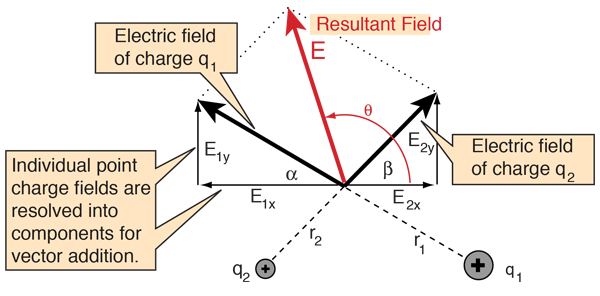
\includegraphics{Figures/electric_field_superposition.png}
    \caption{How to combine two electric fields using vector sums.
    You do not need to know this.
    Image from HyperPhysics.
        \cite{hyperphysics}
    }
    \label{fig:electric_field_superposition}
\end{figure}

    \pnp
    More importantly, we should know that when electric fields point in the same direction, they build each other up,
    while when they point in opposite directions, they work against each other.

    \pnp

    Electric fields give us an easy way to solve the challenge problems from the electric potential section.

    \begin{exboxed}[Exercise~\ref{exr:number_line_1}]
        A positive charge and a negative charge are on a number line as shown.
        Then, you add a positive charge at Point $P$.
        Will the new positive charge move, and if so,
        in which direction?

        \medskip

        \tikzset{every picture/.style={line width=0.75pt}} %set default line width to 0.75pt

\begin{tikzpicture}[x=0.75pt,y=0.75pt,yscale=-1,xscale=1]
%uncomment if require: \path (0,300); %set diagram left start at 0, and has height of 300

%Straight Lines [id:da8648372319496271]
    \draw    (100,222) -- (559.3,222) (142,218) -- (142,226)(184,218) -- (184,226)(226,218) -- (226,226)(268,218) -- (268,226)(310,218) -- (310,226)(352,218) -- (352,226)(394,218) -- (394,226)(436,218) -- (436,226)(478,218) -- (478,226)(520,218) -- (520,226) ;
    \draw [shift={(562.3,222)}, rotate = 180] [fill={rgb, 255:red, 0; green, 0; blue, 0 }  ][line width=0.08]  [draw opacity=0] (10.72,-5.15) -- (0,0) -- (10.72,5.15) -- (7.12,0) -- cycle ;
    \draw [shift={(97,222)}, rotate = 0] [fill={rgb, 255:red, 0; green, 0; blue, 0 }  ][line width=0.08]  [draw opacity=0] (10.72,-5.15) -- (0,0) -- (10.72,5.15) -- (7.12,0) -- cycle ;
%Shape: Circle [id:dp525147663907922]
    \draw  [color={rgb, 255:red, 208; green, 2; blue, 27 }  ,draw opacity=1 ][fill={rgb, 255:red, 208; green, 2; blue, 27 }  ,fill opacity=1 ] (132,221.8) .. controls (132,216.17) and (136.57,211.6) .. (142.2,211.6) .. controls (147.83,211.6) and (152.4,216.17) .. (152.4,221.8) .. controls (152.4,227.43) and (147.83,232) .. (142.2,232) .. controls (136.57,232) and (132,227.43) .. (132,221.8) -- cycle ;
%Shape: Circle [id:dp6232351980171478]
    \draw  [draw opacity=0][fill={rgb, 255:red, 74; green, 144; blue, 226 }  ,fill opacity=1 ] (513,221.8) .. controls (513,216.17) and (517.57,211.6) .. (523.2,211.6) .. controls (528.83,211.6) and (533.4,216.17) .. (533.4,221.8) .. controls (533.4,227.43) and (528.83,232) .. (523.2,232) .. controls (517.57,232) and (513,227.43) .. (513,221.8) -- cycle ;
%Shape: Circle [id:dp8414250651719695]
    \draw  [fill={rgb, 255:red, 0; green, 0; blue, 0 }  ,fill opacity=1 ] (327.24,221.58) .. controls (327.11,219.22) and (328.92,217.22) .. (331.28,217.11) .. controls (333.64,217.01) and (335.67,218.84) .. (335.8,221.2) .. controls (335.93,223.56) and (334.13,225.56) .. (331.76,225.67) .. controls (329.4,225.77) and (327.38,223.94) .. (327.24,221.58) -- cycle ;

% Text Node
    \draw (134+.8,210+5) node [anchor=north west][inner sep=0.75pt]   [align=left] {\textcolor[rgb]{1,1,1}{+}};
% Text Node
    \draw (514+1.5,209+6) node [anchor=north west][inner sep=0.75pt]  [color={rgb, 255:red, 255; green, 255; blue, 255 }  ,opacity=1 ] [align=left] {$\displaystyle -$};
% Text Node
    \draw (335.8,195.2) node [anchor=north west][inner sep=0.75pt]   [align=left] {Point P};


\end{tikzpicture}

    \end{exboxed}

    The electric field caused by the red positive charge and the electric field caused by the blue negative charge both point right
    (which is towards the blue negative charge and away from the red positive charge).
    Since the charge we add to Point $P$ is positive, it travels along the electric field lines and moves right.

    \begin{exrboxed}[Exercise~\ref{exr:number_line_2}]
        Two positive charges of equal magnitude (value) are on a number line as shown.
        Then, you add a negative charge at Point $P$.
        Will the new negative charge move, and if so,
        in which direction? \hint{\ref{hint:number_line}}

        \medskip

        \tikzset{every picture/.style={line width=0.75pt}} %set default line width to 0.75pt

\begin{tikzpicture}[x=0.75pt,y=0.75pt,yscale=-1,xscale=1]
%uncomment if require: \path (0,300); %set diagram left start at 0, and has height of 300

%Straight Lines [id:da8779501834591339]
    \draw    (103,108) -- (562.3,108) (145,104) -- (145,112)(187,104) -- (187,112)(229,104) -- (229,112)(271,104) -- (271,112)(313,104) -- (313,112)(355,104) -- (355,112)(397,104) -- (397,112)(439,104) -- (439,112)(481,104) -- (481,112)(523,104) -- (523,112) ;
    \draw [shift={(565.3,108)}, rotate = 180] [fill={rgb, 255:red, 0; green, 0; blue, 0 }  ][line width=0.08]  [draw opacity=0] (10.72,-5.15) -- (0,0) -- (10.72,5.15) -- (7.12,0) -- cycle ;
    \draw [shift={(100,108)}, rotate = 0] [fill={rgb, 255:red, 0; green, 0; blue, 0 }  ][line width=0.08]  [draw opacity=0] (10.72,-5.15) -- (0,0) -- (10.72,5.15) -- (7.12,0) -- cycle ;
%Shape: Circle [id:dp23414922521798065]
    \draw  [color={rgb, 255:red, 208; green, 2; blue, 27 }  ,draw opacity=1 ][fill={rgb, 255:red, 208; green, 2; blue, 27 }  ,fill opacity=1 ] (135,107.8) .. controls (135,102.17) and (139.57,97.6) .. (145.2,97.6) .. controls (150.83,97.6) and (155.4,102.17) .. (155.4,107.8) .. controls (155.4,113.43) and (150.83,118) .. (145.2,118) .. controls (139.57,118) and (135,113.43) .. (135,107.8) -- cycle ;
%Shape: Circle [id:dp46731974346357785]
    \draw  [color={rgb, 255:red, 208; green, 2; blue, 27 }  ,draw opacity=1 ][fill={rgb, 255:red, 208; green, 2; blue, 27 }  ,fill opacity=1 ] (516,107.8) .. controls (516,102.17) and (520.57,97.6) .. (526.2,97.6) .. controls (531.83,97.6) and (536.4,102.17) .. (536.4,107.8) .. controls (536.4,113.43) and (531.83,118) .. (526.2,118) .. controls (520.57,118) and (516,113.43) .. (516,107.8) -- cycle ;
%Shape: Circle [id:dp6093593677654638]
    \draw  [fill={rgb, 255:red, 0; green, 0; blue, 0 }  ,fill opacity=1 ] (267.24,107.58) .. controls (267.11,105.22) and (268.92,103.22) .. (271.28,103.11) .. controls (273.64,103.01) and (275.67,104.84) .. (275.8,107.2) .. controls (275.93,109.56) and (274.13,111.56) .. (271.76,111.67) .. controls (269.4,111.77) and (267.38,109.94) .. (267.24,107.58) -- cycle ;

% Text Node
    \draw (137+.8,96+5) node [anchor=north west][inner sep=0.75pt]   [align=left] {\textcolor[rgb]{1,1,1}{+}};
% Text Node
    \draw (518+.8,96+5) node [anchor=north west][inner sep=0.75pt]   [align=left] {\textcolor[rgb]{1,1,1}{+}};
% Text Node
    \draw (275.8,81.2) node [anchor=north west][inner sep=0.75pt]   [align=left] {Point P};


\end{tikzpicture}
    \end{exrboxed}

    \subsubsection{Electric Field Lines}\label{subsec:electric-field-lines}

    Electric field lines are just a way to draw the electric field.
    The direction of the lines is the direction of the electric field,
    and the more lines in a given region, the stronger the field.
    A positive charge travels along the electric field lines,
    while a negative charge travels against them.
    Electric field lines point in the direction of decreasing potential.
    \begin{figure}
    \centering
    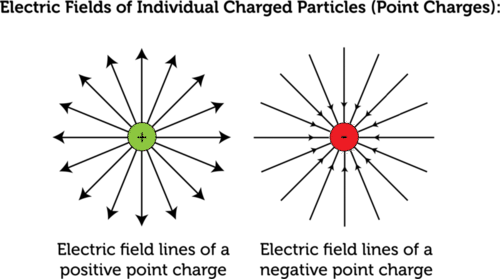
\includegraphics[width=.8\textwidth]{Figures/electric_field_point_charge.png}
    \caption{The electric field lines caused by individual charges.
    Image from CK-12 Foundation under CC BY-NC 3.0.
        \cite{ck12}}
    \label{fig:electric_field_point_charges}
\end{figure}


    \begin{exrboxed}
        A negatively charged object is placed in an electric field pointing left.
        In which direction does the object move?
    \end{exrboxed}

    Since a negative charge moves against the electric field lines,
    the object will move right.


    \begin{figure}
    \centering
    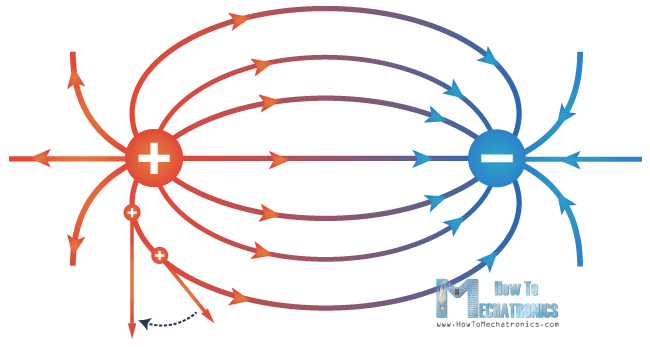
\includegraphics[width=.8\textwidth]{Figures/dipole}
    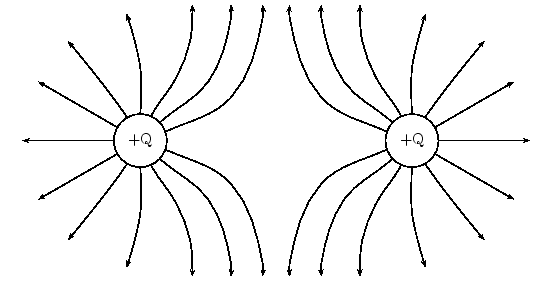
\includegraphics[width=.8\textwidth]{Figures/like_positive}
    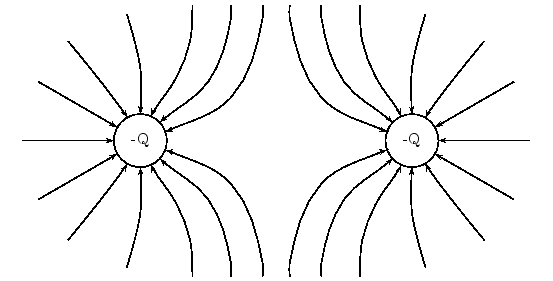
\includegraphics[width=.8\textwidth]{Figures/like_negative}
    \caption{Electric field lines for different systems of two particles.
    Images from How To Mechatronics~\cite{htm} and Riaan at English Wikibooks / GFDL~\cite{like_pos,like_neg}}.
    \label{fig:field_lines}
\end{figure}




    \begin{mdframed}[style=exmdbox]
        \begin{problem}
            What is the electric field strength at a point $7\meters$ from a $-2.2\coulombs$ charge?
            What direction is the electric field (away from the charge, towards the charge, or something else)?
        \end{problem}
        \begin{problem}
            What is the electric field strength $2\millimeters$ from a charge of $6.4\nanocoulombs$? \hint{\ref{hint:table_of_conversions}}
        \end{problem}

        \begin{problem}
            What happens to electric field strength as the distance to the charge decreases? \hint{\ref{hint:approximate_limit_electric_field}}
        \end{problem}

        \begin{problem}[Challenge]
            Point $P$ is 10 meters to the right of an unknown charge.
            The electric potential at Point $P$ is $3\volts$.
            What is the electric field (strength and direction) at Point $P$? \hint{\ref{hint:field_challenge_1}}
        \end{problem}

    \end{mdframed}


    \section{Electric Force (Coulomb's Law)}
    We said that the electric field is the direction a positively charged particle will move when released
    and how strong the difference in potential is.
    However, how much a particle is affected by the field depends on the charge of that particle.

    \pnp

    An electric field induces more force on a particle with a large charge than one with a small charge.
    In fact, you can think of electric field as force per unit charge.

    \begin{thmboxed}
        The electric field is equal to force per unit charge,
        so
        \begin{equation}
            E=\frac{F}{q}.
            \label{eq:force_per_unit_charge}
        \end{equation}
    \end{thmboxed}

    \begin{exboxed}
        If the electric field strength $E$ at a point is $10 \newtonsspercoulomb$,
        what force would a $1 \coulombs$ charge experience if placed at that point?
    \end{exboxed}

    We use Equation~\ref{eq:force_per_unit_charge} to find that
    \begin{align*}
        F &= E\cdot q\\
        &= 10 \newtonspercoulomb \cdot 1 \coulombs\\
        &= \boxed{10 \newtons}.
    \end{align*}

    \pagebreak[2]
    \begin{thmboxed}[Coulomb's Law]
        The electric field is equal to force per unit charge,
        so
        \begin{align*}
            F &= E\cdot q\\
            F &= \del{\frac{kQ}{r^2}}\cdot q\\
            F &= k\frac{qQ}{r^2}.
        \end{align*}
    \end{thmboxed}

    \begin{mdframed}[style=exmdbox]
        \begin{problem}
            If a $-10 \coulombs$ charge at Point $P$ experiences an electric force of magnitude $530\newtons$,
            what is the electric field strength at Point $P$?
        \end{problem}

        \begin{problem}
            How far must a $2\nanocoulombs$ charge be from a $1\microcoulombs$ charge such that the force between them\footnotemark{} is $3.4\newtons$?
            \hint{\ref{hint:table_of_conversions}}
        \end{problem}

        \begin{problem}[Shieh]
            Two charges are placed next to each other.
            Both charges have a charge of $8.3\times10^{-11}\coulombs$ and the distance between them is $5.7\times10^{-5}\meters$.
            What is the electrical force?
        \end{problem}

        \begin{problem}[Shieh]
            Two charges are separated by $3.5\times10^{-5}\meters$.
            The first charge has a charge of $7.2\times10^{-10}\coulombs$,
            and the second has a charge of $-1.6\times10^{-10}\coulombs$.
            What is the electrical force between them?
        \end{problem}
    \end{mdframed}
    \footnotetext{The force between any two charges is equal to the force either one of them imposes on the other.
    By Newton's Third Law of Motion, the force will be the same no matter which particle you choose.}


    \section{Potential Energy}\label{sec:potential-energy}

    Like the electric force is charge times electric field (Equation~\ref{eq:force_per_unit_charge}: $F=q\cdot E$),
    electric potential energy ($U$) is charge times electric potential.
    % remove next sentence?
    In that sense, electric potential is a form of potential energy per unit charge.

    \begin{thmboxed}
        Electric potential is equal to electric potential energy per unit charge,
        so
        \begin{equation}
            V=\frac{U}{q}.
            \label{eq:potential_per_unit_charge}
        \end{equation}
    \end{thmboxed}

    \begin{exboxed}
        If the electric potential $V$ at a point is $7 \volts$,
        how much potential energy would a $0.4 \coulombs$ charge have at that point?
    \end{exboxed}

    We use Equation~\ref{eq:potential_per_unit_charge} to find that
    \begin{align*}
        U &= V\cdot q\\
        &= 7 \volts \cdot 0.4 \coulombs\\
        &= \boxed{2.8 \joules}.
    \end{align*}

    \pagebreak[2]
    \begin{thmboxed}
        Electric potential is equal to electric potential energy per unit charge,
        so
        \begin{align*}
            U &= V\cdot q\\
            U &= \del{\frac{kQ}{r}}\cdot q\\
            U &= k\frac{qQ}{r}.
        \end{align*}
    \end{thmboxed}

    \begin{exercises}
        \begin{problem}
            A system of two point charges has $U=-1.41\times 10^{-6} \joules$.
            If the first charge is $-25\coulombs$ and the second is $27 \coulombs$,
            what is the distance between the charges?
        \end{problem}
        \begin{problem}[Challenge]
            Assume a charge $+Q$ is fixed in place.
            A charge $+q$ is released from rest from a distance of $10\nanometers$ away from $Q$.
            Because both charges are positive, they repel each other and the $+q$ charge starts to move further away from the fixed $+Q$ charge.
            What is the total energy of the $+q$ charge once it is $30\centimeters$ away from the $+Q$ charge?
            \hints{\ref{hint:table_of_conversions}, \ref{hint:conservation_of_energy}, \ref{hint:zero_kinetic_energy}}
        \end{problem}
    \end{exercises}

    \subsubsection{Work}
    Just as voltage is the difference in potential between two points ($\Delta V$),
    work is the difference in potential energy of a particle between two points ($W=\Delta U$).

    \pnp

    Since $U=V\cdot q$,
    \begin{align*}
        \Delta U&=\Delta \del{V\cdot q}\\
        &= \del{\Delta V}\cdot q.\: \footnotemark
    \end{align*}
    \footnotetext{Technically, $\Delta \del{V\cdot q}$ equals $\del{\Delta V}\cdot q+\del{\Delta q}\cdot V+\del{\Delta V}\del{\Delta q}$,
    but we make the assumption that charge doesn't change ($\Delta q=0$) to simplify to $\del{\Delta V}\cdot q$.}


    \section{Ratio Trick}\label{sec:ratio-trick}
    When we're asked what would happen if we scaled some variables by a constant,
    the answer would be the same no matter what the original values of the variables are\footnote{This is only true if the only operations are addition and multiplication.}.

    \pnp

    So, we can set the original values of the variables to whatever number we choose.
    Since both multiplication and division by 1 don't change the number,
    it will make our lives easier if we choose all of them to be 1.

    \pnp

    Then, the original number is 1 while the final number is just the ratio of scaling factors.
    Let's look at an example to make this more clear.

    \begin{exboxed}
        What happens to the electric field as $Q$ doubles and $r$ triples?
        \label{ex:ratio-trick}
    \end{exboxed}

    Remember that by Equation~\ref{eq:electric-field},
    $E=\frac{kQ}{r^2}$.
    First we check to make sure that our equation involves only multiplication and division.
    Since this equation only involves mutiplication and division,
    we can use the ratio trick.

    \pnp

    Plugging in 1 for all the initial variables,
    we get
    \[E_{\text{initial}}=\frac{1\cdot1}{1^2}=1.\]
    In fact, the initial value will \emph{always} equal 1 with this trick.
    Then, we plug in the scaled versions of the variables:
    \[E_{\text{scaled}}=\frac{1\cdot2}{3^2}=\frac{2}{9}.\]
    We find that what happens to $E$ as $Q\mapsto2Q$ and $r\mapsto3r$ is that $E$ gets multiplied by $\frac{\frac{2}{9}}{1}=\frac{2}{9}$,
    or $\boxed{E\mapsto\frac{2}{9}E}$.

    \subsubsection{Shortcut}

    There is an even shorter and simpler version of the ratio trick.
    We only need to calculate the scaled variable as in $E_\text{scaled}$ from Section~\ref{sec:ratio-trick}.
    This is easy, we just
    \bluebf{plug in the scaling factor for every variable that changes and 1 for everything that doesn't.}

    \pnp

    Using Example~\ref{ex:ratio-trick},
    we again get \[E_{\text{scaled}}=\frac{1\cdot2}{3^2}=\frac{2}{9}.\]
    This immediately tells us that $\boxed{E\mapsto\frac{2}{9}E}$.

    \begin{mdframed}[style=exmdbox, frametitle={Exercises from Mr. Shieh}]
        \begin{problem}[Shieh]
            When $q$ increases by a factor of 5, how does $F$ change?
        \end{problem}
        \begin{problem}[Shieh]
            When $k$ decreases by a factor of 2, how does $F$ change?
            \hints{\ref{hint:k_changes}, \ref{hint:decrease_by_a_factor}}
        \end{problem}
        \begin{problem}[Shieh]
            When $r$ increases by a factor of 3, how does $F$ change?
        \end{problem}
    \end{mdframed}

    \pagebreak[3]


    \section{Equations to Remember}\label{sec:equations-to-remember}

    Everything that we have learned can be derived from the following equations.

    \par

    {\Large
        \begin{align*}
            \setlength{\abovedisplayskip}{3em}
            \setlength{\belowdisplayskip}{\abovedisplayskip}
            V&=\frac{kQ}{r} & U=q\cdot V\\
            E&=\frac{kQ}{r^2} & F=q\cdot E
        \end{align*}}%




    \pagebreak[4]


    \section{Hints} \label{sec:hints}

    \begin{enumerate}[leftmargin=0pt, itemsep=1.4em]

        \item \label{hint:voltage_challenge_1} It is, in fact, impossible to find out what $V$ and $r$ are.
        However, we can find out the value they have when multiplied together, $V\cdot r$.
        This will allow you to find $Q$, the desired value of the charge.
        \item \label{hint:circle1} A circle has a constant radius.
        That is, the distance $r$ to the circle's center is the same from every point on the circle.
        \item \label{hint:k_changes} This can never actually happen in real life because $k$ is a constant.
        Still, you can answer the question using the trick from Section~\ref{sec:ratio-trick}.
        \item \label{hint:circle2} The charge $Q$ in the center of the circle and the constant $k$ don't change.
        What does that mean in your formulae?
        \item \label{hint:ex} This is an example of a hint.
        \item \label{hint:number_line} The electric field caused by the charge on the left points right, while the electric field caused by the charge on the right points left.
        This means that they will work against each other.
        Which of the electric fields is stronger?
        \item \label{hint:table_of_conversions} Use your table of conversions provided by Mr. Shieh or \href{https://physics.nist.gov/cuu/Units/prefixes.html}{this one} to convert to SI base units.
        Then solve as normal.
        \item \label{hint:decrease_by_a_factor} To decrease by a factor of $s$ means to multiply by $1/s$.
        For example, decreasing by a factor of 10 is the same as being multiplied by $1/10=0.1$.
        \item \label{hint:field_challenge_1} What is the equation for potential?
        What is the equation for electric field strength?
        How are they related?
        \item \label{hint:conservation_of_energy} We can use the Law of Conservation of Energy,
        which says that the total energy of any closed system remains the same over time.
        Because of that, you just need to calculate total energy for whichever point in time is most convenient.
        \item \label{hint:approximate_limit} Try plugging in larger and larger values of $r$ and see what happens to $V$.
        \item \label{hint:zero_kinetic_energy} The only energies that we need to consider are kinetic energy (energy from motion) and electric potential energy.
        When the charge $+q$ is at rest (before it is released and starts to shoot away from the $+Q$ charge),
        it is not moving (this is the definition of rest), so it has no kinetic energy.
        This means that the total energy is just the electric potential energy at this time.
        \item \label{hint:approximate_limit_electric_field} Try plugging in smaller and smaller values of $r$ and see what happens to $E$.
    \end{enumerate}
    \bibliographystyle{plain}
    \bibliography{ref}
    \subsubsection*{Acknowledgements}
    The styles for this worksheet are based on styles created by CJ Quines.
\end{document}
